\chapter{ Implémentation d'agent }
\label{Implementation_d_agent}
\paragraph{}
Les agents sont considérés comme l'un des paradigmes les plus importants qui peuvent améliorer les méthodes actuelles de conceptions. Le terme "Agent" a trouvé son chemin dans un certain nombre de technologie et a été largement utilisé, par exemple, dans l'intelligence artificielle, les bases de données, les systèmes d'explorations, etc. Un agent est essentiellement un composant logiciel spécial qui possède une autonomie. Un agent est un systèm solidaire qui travail dans un environnement. Les systèmes multi-agents peuvent modéliser des systèmes complexes. les agents dans ce système agisse les un sur les autres. Un agent est autonome et proactif qu'il n'agit pas simplement en réponse à son environnement mais est capable d'afficher un comportement orienté vers l'objectif en prenant l'initiative (autonomous behavior).

\section{ Jade }
\subsection{Jade architecture}
\paragraph{}
Jade est composée de conteneurs d'agents qui peuvent être distribués sur le réseau. Les agents vivent dans des conteneurs qui sont le processus java qui fournit le temps d'exécution de JADE et tous les services nécessaires pour héberger et exécuter des agents. Il y a un conteneur spécial, appelé conteneur principal, qui représente le point d'amorçage d'une plate-forme: c'est le premier conteneur à lancer et tous les autres conteneurs doit se joindre à un conteneur principal (main container) en s'inscrivant avec lui.
\paragraph{}
JADE est un middleware qui facilite le développement de systèmes multi-agents en vertu de la norme FIPA pour laquelle il crée de multiples conteneurs pour les agents, chacun d'eux peut fonctionner sur un ou plusieurs systèmes. Il est entendu qu'un ensemble de conteneurs constitue une plate-forme.

JADE propose:
\begin{itemize}
    \item Un environnement où les agents JADE sont exécutés.
    \item Bibliothèques pour créer des agents utilisant l'héritage et la redéfinition des comportements.
    \item Une boîte à outils graphique pour le suivi et la gestion de la plate-forme d'agents intelligents.

\end{itemize}


\subsection{Le cycle de vie d'agent JADE}
\paragraph{}
Le cycle de vie d'un agent JADE suit le cycle proposé par FIPA. Ces agents passent par différents états définis comme:
\begin{itemize}

    \item Initié: l'agent a été créé.
    \item Active: L'agent a été enregistré et a un nom. Dans cet état, il peut communiquer avec d'autres agents.
    \item Suspendu: l'agent est arrêté parce que son thread est suspendu.
    \item Attente: l'agent est bloqué en attente d'un événement.
    \item Supprimé: L'agent a terminé et son thread a terminé son exécution.
    \item Transit: l'agent se déplace vers un nouvel emplacement.
\end{itemize}

\paragraph{}
\section{Gui Agent}
Dans notre application, l'interface graphique est un agent. Cet agent au moment d'initialisation il crée un conteneur d'agent "sink-container". Ce contenair servira comme bassin pour les controlleurs ( chaque module; atome, molécule et réaction; est un agent sont missions principales est d'assurer le bon déroulement de la simulation.


\usetikzlibrary{arrows.meta}
\tikzset{%
  >={Latex[width=2mm,length=2mm]},
  % Specifications for style of nodes:
            base/.style = {rectangle, rounded corners, draw=black,
                           minimum width=4cm, minimum height=1cm,
                           text centered, font=\sffamily},
  activityStarts/.style = {base, fill=blue!30},
       startstop/.style = {base, fill=red!30},
    activityRuns/.style = {base, fill=green!30},
         process/.style = {base, minimum width=2.5cm, fill=orange!15,
                           font=\ttfamily},
}


\begin{lstlisting}

//ApplicationAgent.java
public class ApplicationAgent extends Agent {
    /** setting up agent **/
    @Override
    public void setup() {
        System.setProperty("prism.dirtyopts", "false");
        Application.launch(FactoryGui.class);
    }
}
//FactoryGui.java
public class FactoryGui extends Application {
    /** Gui Agent start : define agent profile, create container for the controllers agents */
    @Override
    public void start(Stage stage) throws Exception {
        Runtime rt = Runtime.instance();
        /.../
        pc.setParameter(Profile.LOCAL_HOST, "127.0.0.1");
        pc.setParameter(Profile.CONTAINER_NAME, "sink-container");
        pc.setParameter(Profile.NO_MTP, "true");
        AgentContainer container = rt.createAgentContainer(pc);
        /.../
            FXMLLoader f = new // setting up the Gui FXMLLoader(ApplicationAgent.class.getClassLoader().getResource(("uiAtoms.fxml")));
            Parent parent = f.load();
            c = f.getController();
            c.setParent(parent);
            c.setContainer(container);//creating controllers container
            container.acceptNewAgent("controller", c);//adding main controller in the container
            c.AStart(stage, true);
            /.../

    }
}
\end{lstlisting}

\section{Controller agent}
\paragraph{}
Le main controlleur a pour mission le bon fonctionnement de GUI, il initialise les autres controlleurs (chaque tab a son propre controlleur qui assure le fonctionnement de ce tab). Ces controlleurs créer les environnements ou se déroulera la réaction. Chaque environnement est un container qui recevra les différents atomes sous forme d'agent.



\begin{tikzpicture}[node distance=1.5cm,
    every node/.style={fill=white, font=\sffamily}, align=center]

  \node (start)             [Application]              {Application agent starts};
  \node (masterController)     [process, below of=start]          {Controller (MASTER)};
  \node (AtomController)      [process,below of=masterController, right of=ReactionController , xshift=-6cm]   {Atom Controller};
  \node (MolecularController)      [process,below of=masterController, left of=ReactionController, xshift=6 cm]   {Molecule Controller};
  \node (ReactionController)      [process, below of=masterController]   {Reaction Controller};

  \node (atom1)     [process, below of=AtomController]   {Atom ex: H};
  \node (Environment)      [activityRuns, below of=ReactionController]
                                                      {Create Environment};

  \node (atoms)     [activityRuns, yshift=-2cm, below of=Environment]   {Atoms as agents};


  \draw[->]     (start) -- (masterController);
  \draw[->]     (masterController) -- (AtomController);
  \draw[->]     (masterController) --(MolecularController);
  \draw[->]     (masterController) --  (ReactionController);
  \draw[->]     (ReactionController) --  (Environment);
  \draw[->]     (MolecularController) |-  (Environment);
  \draw[->]     (AtomController) --  (atom1);
  \draw[->]     (atom1) |- node[text width=3cm]
                                   {Add atom to environment}  (Environment);
  \draw[->]     (Environment) -- node[text width=3cm]
                                   {contain agents}(atoms);

  \end{tikzpicture}

\section{Atom agent}
\paragraph{}
Chaque atome dans notre application est considéré comme un agent. Il a un cycle de vie composé de quatres phase:
\begin{itemize}
\item Phase d'initialisation (setup) : dans laquelle, l'atome initialise ces propriétés (vitesse, symbole, rayon de van der waals ...)
\item Phase de démarrage : dans la quelle il va rejoindre le conteneur d'agent est déclenché son comportement.
\item Phase de vitalité : dans la quelle l'atome a son propre comportement selon un modèle chimico-physique à l'aide des différent algorithme a bordé dans la section simulation moléculaire.
\item Phase de destruction : l'agent sera retiré du conteneur d'agent et détruit de la simulation. 
\end{itemize}


\begin{figure}[H]
\centering
\centerline{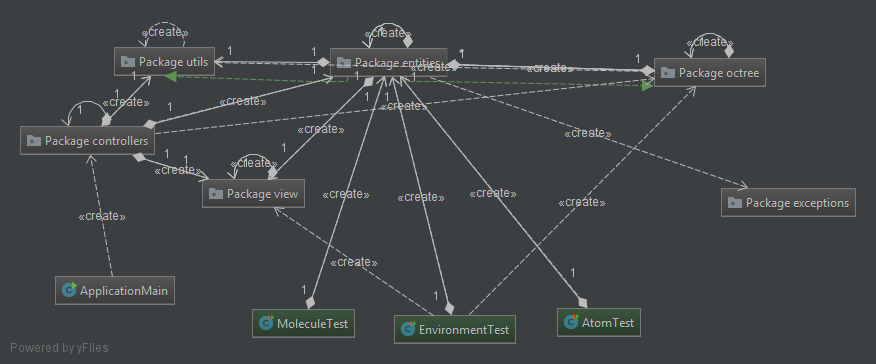
\includegraphics[width=1\textwidth]{diagram.png}}
\caption{Diagrame de dépendenc }
\label{diagram_im}
\end{figure}